\chapter{Restricted Boltmann Machines}
\section{Affrontare i minimi spuri nelle Hopfield Networks}
Utilizzando la regola di storage di Hopfield la capacità di una rete rete completamente connessa con $N$ unità è di appena $0.15N$ ricordi.


\textbf{Ciò rende inefficiente l'utilizzo dei bit richiesti per memorizzare i pesi}. Infatti ogni volta che memorizziamo una configurazione, speriamo di creare un nuovo minimo energetico (uno stato stabile). Ma cosa succede se \textbf{due minimi vicni si uniscono per creare un minimo in un punto intermedio}? In realtà è questo a limitare la capacità della Hopfield net.
\begin{figure}[!h]
    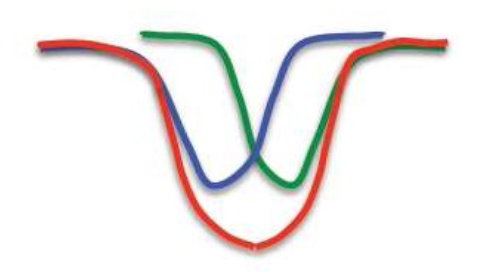
\includegraphics[scale=1]{images/rbm/minimum.png}
    \centering
\end{figure}


\begin{figure}
\centering     %%% not \center
\subfigure[Set di pattern fatti a mano per un esperimento con Hopfield net]{\label{fig:a}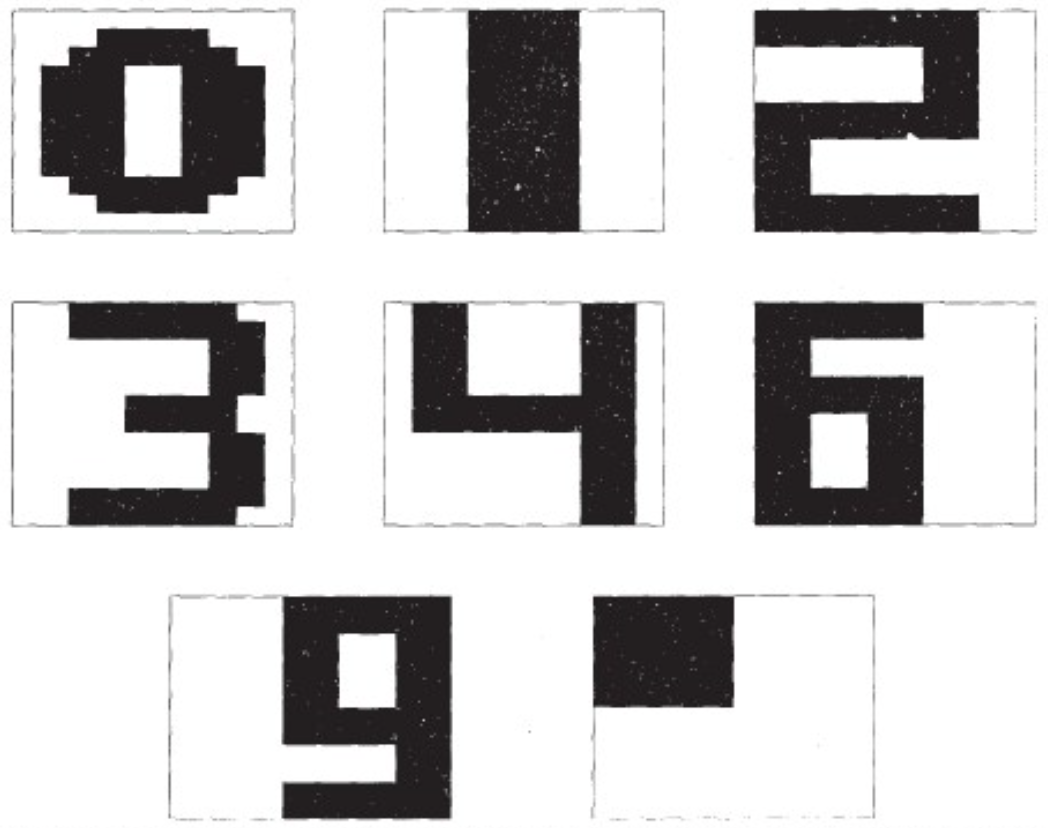
\includegraphics[width=60mm,height=60mm]{images/rbm/pt01.png}}
\subfigure[Compilation di stati spuri prodotti durante l'esperimento]{\label{fig:b}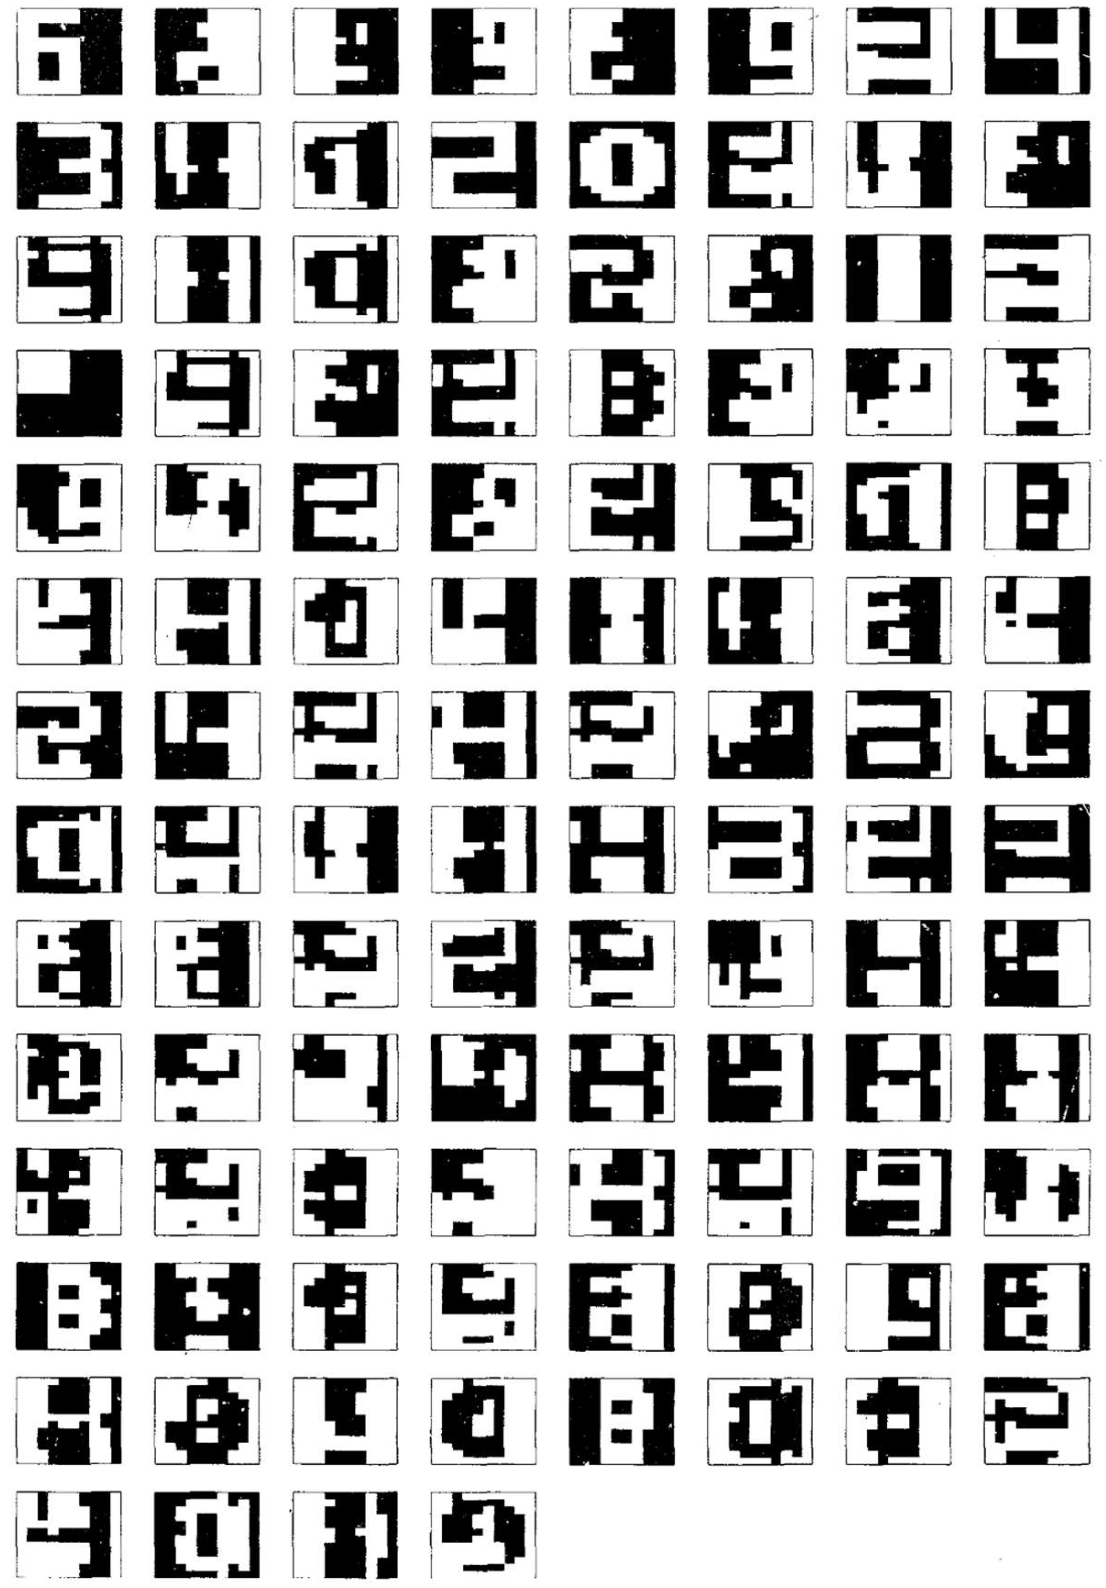
\includegraphics[width=60mm,height=60mm]{images/rbm/pt02.png}}
\end{figure}
\newpage
I fisici hanno a lungo studiato come aumentare la capacità di storage delle Hopfield net. 



Hopfield, Feinstein e Palmer suggerirono la seguente strategia:
\begin{itemize}
    \item lascia che la rete si stabilizzi da uno stato iniziale casuale e poi fai un \textbf{unlearning};
    \item questo eliminerà i profondi minimi spuri e aumenterà la capacità di memoria.
\end{itemize}
Hanno dimostrato che effettivamente funziona. Ma \textbf{non l'hanno analizzato}.

Crick e Mitchinson proposero l'unleraning come modello di ciò a cui servono i sogni. Ma la domanda è \textit{quanto unlearning dovremmo fare?} Si può utilizzare unlearning per minimizzare una qualche funzione costo?


A questo punto si avevano tre idee principali:
\begin{itemize}
    \item visible vs invisible units;
    \item stochastic units;
    \item un nuovo algoritmo per correggere gli errori.
\end{itemize}
\newpage
\section{RBM}
\begin{figure}[!h]
    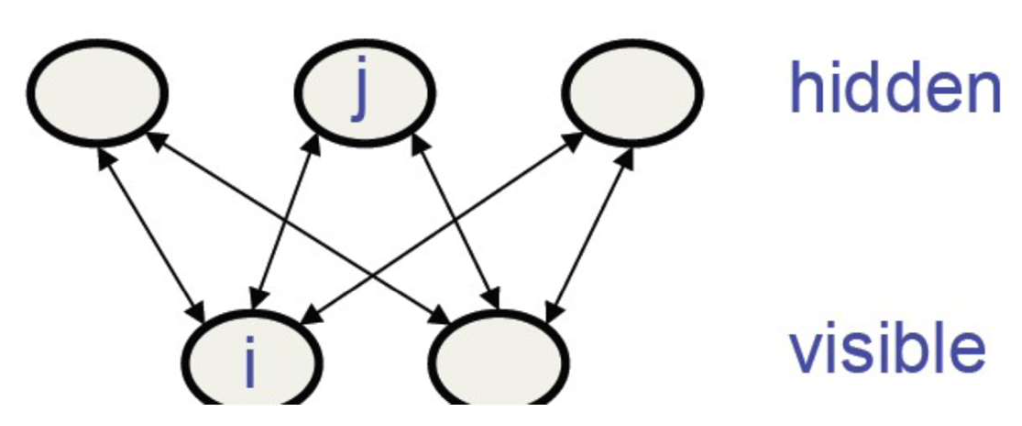
\includegraphics[scale=.8]{images/rbm/rbm.png}
    \centering
\end{figure}


Sono presenti connessioni solo tra unità visibili e hidden: tutte le unità visibili sono connesse a tutte le unità hidden.



I pesi sono simmetrici quindi $w_{ij}=w_{ji}$.


I possibili stati di attivazione dei neuroni sono $0$ o $1$.



I neuroni sono stocastici.
\newline
\newline
Presentare un \textbf{input} ad una RBM significa imporre una \textbf{configurazione di attivazioni alle unità nel visual layer che corrisponde all'ipnut}. A quel punto l'RBM genera un \textbf{output} al livello visibile: questo rappresenta \textbf{il pattern delle  attivazioni delle unità visibili}.


Invece di utilizzare la rete per conservare memories, la si usa per \textbf{costruire interpretazioni del sensore di input}. L'input è rappresentato dalle \textbf{unità visibili}. L'interpretazione è rappresentata dagli \textbf{stati delle unità hidden}.



\textbf{Costruire interpretazioni} significa \textbf{individuare e rappresentare le regolarità nelle visual activations}. Le hidden units si specializzano nel riconoscimento (e nella generazione) delle porzioni di pattern visuali.
\subsection{Stochastic neurons}
Il punto fondamentale è che le \textbf{reti rumorose trovano minimi energetici migliori}. Una Hopfield net prende sempre le decisioni in ottica di riduzione dell'energia e ciò rende impossibile evitare un \textbf{minimo locale}.
\begin{figure}[!h]
    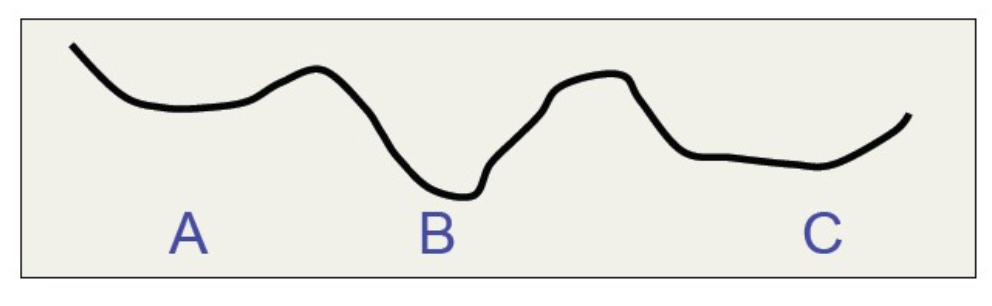
\includegraphics[scale=.8]{images/rbm/local_minima.png}
    \centering
\end{figure}
\newpage
Rimpiazziamo le unità di treshold binarie con unità stocastiche binarie che prendono decisioni casuali biased. La \textbf{temperatura} controlla l'ammontare di rumore.
\begin{equation}
    p\big( s_i=1 \big) = \frac{1}{1+e^{-\Delta \frac{E_i}{T}}}.
\end{equation}
\begin{figure}[!h]
    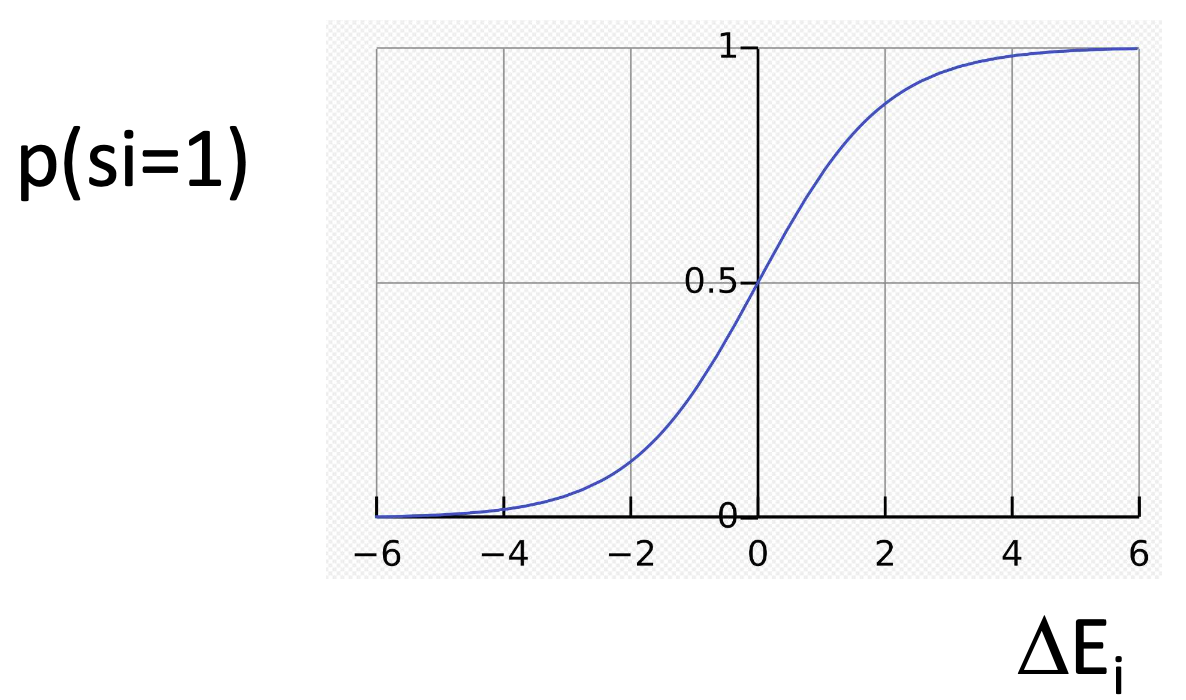
\includegraphics[scale=.5]{images/rbm/temp.png}
    \centering
\end{figure}


\begin{equation}
    \text{Energy gap }=\Delta E_i = E\big( s_i=0 \big)-E\big( s_i=1 \big),
\end{equation}
\begin{equation}
    E = -\sum_k\sum_jw_{jk}v_kh_j,
\end{equation}
\begin{equation}
   \Delta E_i=\sum w_{ij}s_j, \forall j \text{ connesso ad } i.
\end{equation}
In questo contesto $T=$ temperature. Consideriamo sempre $T=1$, perciò lo ignoreremo.
Inoltre:
\begin{itemize}
    \item $s_i\in(0,1)$ è l'activation state del genrico neurone $i$;
    \item $v_i$ come $s_i$ limitato alle unità visibili;
    \item $h_j$ come $s_i$ limitato alle unità hidden.
\end{itemize}
Una volta che è stato calcolato $P(h_1=1)$, o una distribuzione di probabilità per molte unità in parallelo, \textbf{campioniamo}  per attribuire uno stato di $0$ o $1$ utilizzando la probabilità.
\newline
\newline
Perciò il ciclo è il seguente:
\begin{itemize}
    \item arriva un visual input;
    \item calcolo l'attivazione all'hidden level;
    \item ricalcolo l'attivazione al livello visuale;
    \item possibilmente ricominciare.
\end{itemize}
\newpage
\paragraph{Esercizio.} Calcolare $p(h_1=1)(e^{-0.01}=0.99)$.
\begin{figure}[!h]
    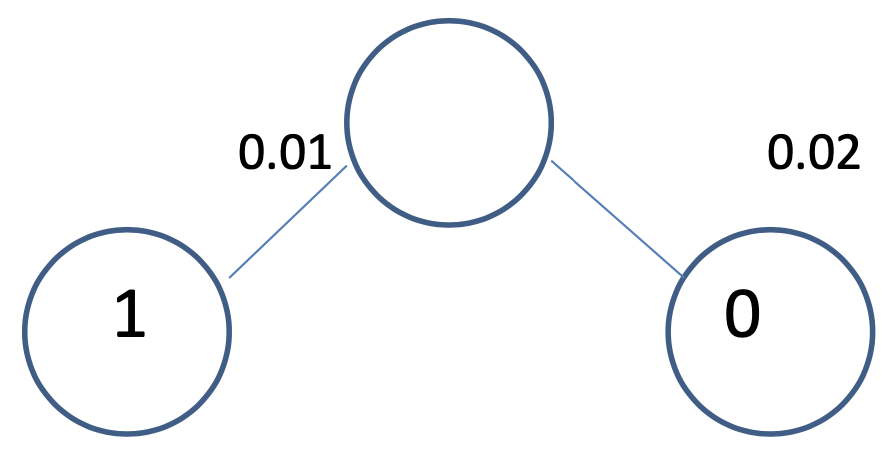
\includegraphics[scale=.4]{images/rbm/ex01.png}
    \centering
\end{figure}


\textbf{Soluzione:}  $P(h_1=1)=0.5025$



A questo punto dobbiamo \textbf{campionare}.
\begin{figure}[!h]
    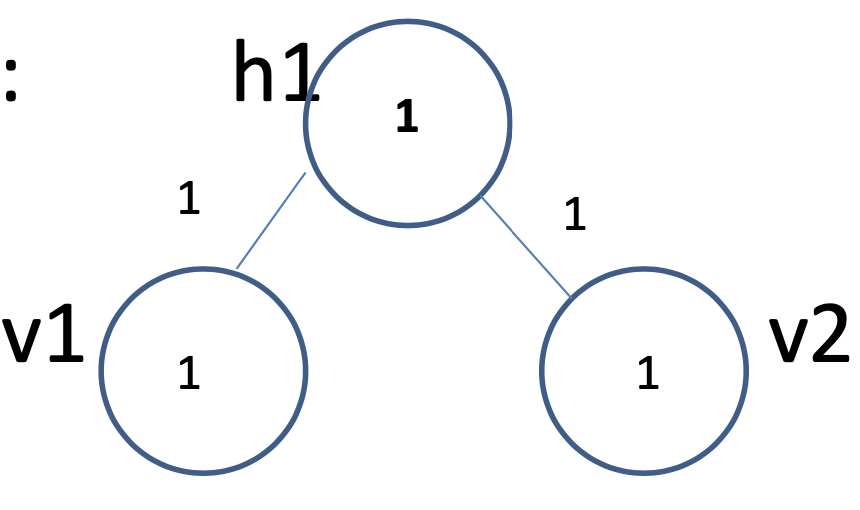
\includegraphics[scale=.4]{images/rbm/ex02.png}
    \centering
\end{figure}
Dati questi pesi, se $v_1=1$ e $v_2=1$
\begin{equation}
    P(h_1=1)=\frac{1}{1+e^{-\Delta E_i}}=\frac{1}{1+e^{-2}}=0.88,
\end{equation}
e campionando, con probabilità $0.88$, avremo $h_1=1$ (l'attivazione di $h_1$ sarà settata a $1$).


A partire poi da $h_1=1$ possiamo ricominciare e ricalcolare $v_1$ e $v_2$:
\begin{equation}
    \begin{split}
        P(v_1=1)=\frac{1}{1+e^{-\Delta E_i}}=\frac{1}{1+e^{-2}}=0.73\\
        P(v_2=1)=\frac{1}{1+e^{-\Delta E_i}}=\frac{1}{1+e^{-2}}=0.73\\
    \end{split}
\end{equation}
campionando abbiamo alta probabilità di avere $v_1=1$ e $v_2=1$.


